\documentclass[12pt,a4paper]{article}

% ─── Page Layout ───────────────────────────────────────────────────────────────
\usepackage[a4paper, margin=0.8in, headheight=14pt]{geometry}

% ─── Fonts (XeLaTeX) ───────────────────────────────────────────────────────────
\usepackage{fontspec}
\usepackage{unicode-math}
\setmainfont{TeX Gyre Pagella}
\setmonofont[Scale=0.88]{TeX Gyre Cursor}
\setmathfont{Latin Modern Math}

% ─── Packages ──────────────────────────────────────────────────────────────────
\usepackage{xcolor}
\usepackage{colortbl}
\usepackage{titlesec}
\usepackage{enumitem}
\usepackage{tabularx}
\usepackage{booktabs}
\usepackage{array}
\usepackage{amsmath}
\usepackage{tikz}
\usetikzlibrary{shapes.geometric, arrows.meta, positioning, calc, fit, decorations.pathreplacing}
\usepackage{tcolorbox}
\tcbuselibrary{skins, breakable}
\usepackage{hyperref}
\usepackage{fancyhdr}
\usepackage{graphicx}
\usepackage{microtype}
\hyphenpenalty=10000
\exhyphenpenalty=10000
\sloppy
\usepackage{caption}
\usepackage{setspace}
\usepackage{multirow}
\usepackage{tocloft}

% ─── Q&A helper ────────────────────────────────────────────────────────────────
\newcommand{\Q}[1]{\textbf{#1}\par\noindent\ignorespaces}

% ─── Colour Palette ────────────────────────────────────────────────────────────
\definecolor{myred}{RGB}{196,30,58}
\definecolor{mydark}{RGB}{30,30,50}
\definecolor{mygreen}{RGB}{14,120,80}
\definecolor{myteal}{RGB}{0,130,140}
\definecolor{myamber}{RGB}{180,100,0}
\definecolor{mypurple}{RGB}{100,30,160}
\definecolor{mygray}{RGB}{246,247,249}
\definecolor{mgframe}{RGB}{180,185,200}
\definecolor{watermark}{RGB}{145,150,170}
\definecolor{hdrred}{RGB}{250,232,235}
\definecolor{hdrgreen}{RGB}{220,244,233}
\definecolor{hdrteal}{RGB}{220,242,244}
\definecolor{hdramber}{RGB}{253,242,215}
\definecolor{hdrpurple}{RGB}{238,228,255}
\definecolor{hdrgray}{RGB}{238,240,245}
\definecolor{rowalt}{RGB}{250,251,253}

% ─── Section Formatting ────────────────────────────────────────────────────────
\titleformat{\section}
  {\large\bfseries\color{myred}}{\thesection.}{0.5em}{}
  [\vspace{1pt}{\color{myred}\rule{\linewidth}{0.8pt}}]
\titleformat{\subsection}
  {\normalsize\bfseries\color{myteal}}{\thesubsection}{0.5em}{}
\titlespacing*{\section}{0pt}{18pt}{7pt}
\titlespacing*{\subsection}{0pt}{11pt}{4pt}

% ─── Paragraph ─────────────────────────────────────────────────────────────────
\setlength{\parindent}{0pt}
\setlength{\parskip}{4pt}

% ─── TOC Styling ───────────────────────────────────────────────────────────────
\renewcommand{\cfttoctitlefont}{\large\bfseries\color{myred}}
\renewcommand{\cftaftertoctitle}{\par\noindent{\color{myred}\rule{\linewidth}{0.8pt}}}
\setlength{\cftbeforetoctitleskip}{0pt}
\setlength{\cftaftertoctitleskip}{6pt}
\renewcommand{\cftsecfont}{\normalsize\bfseries\color{mydark}}
\renewcommand{\cftsecpagefont}{\normalsize\bfseries\color{mydark}}
\renewcommand{\cftsecleader}{\cftdotfill{\cftdotsep}}
\setlength{\cftbeforesecskip}{7pt}
\renewcommand{\cftsubsecfont}{\small\color{mydark}}
\renewcommand{\cftsubsecpagefont}{\small\color{mydark}}
\setlength{\cftbeforesubsecskip}{3pt}
\setlength{\cftsubsecindent}{1.4em}

% ─── Table helpers ─────────────────────────────────────────────────────────────
\renewcommand{\arraystretch}{1.45}
\setlength{\tabcolsep}{6pt}
\arrayrulecolor{mydark}
\newcolumntype{B}[1]{>{\small\bfseries\raggedright\arraybackslash}m{#1}}
\newcolumntype{Y}{>{\small\raggedright\arraybackslash}X}
\renewcommand{\tabularxcolumn}[1]{m{#1}}

% ─── Header / Footer ───────────────────────────────────────────────────────────
\pagestyle{fancy}
\fancyhf{}
\fancyhead[L]{\small\color{myred}\textbf{PE-EC703A}\;\color{mydark}--- Embedded System}
\fancyhead[R]{\small\color{myteal}\textbf{Module 4 Notes}}
\fancyfoot[C]{\small\color{mydark}\thepage}
\fancyfoot[R]{\small\color{watermark}\textit{\copyright\ Biraj}}
\renewcommand{\headrulewidth}{0.5pt}
\renewcommand{\footrulewidth}{0.3pt}

% ─── Hyperref ──────────────────────────────────────────────────────────────────
\hypersetup{
  colorlinks=true, linkcolor=myteal, urlcolor=myteal,
  pdfauthor={Biraj Sarkar},
  pdftitle={PE-EC703A --- Module 4 Notes}
}

% ─── tcolorbox styles ──────────────────────────────────────────────────────────
\tcbset{
  tikzbox/.style={
    colback=mygray, colframe=mgframe, boxrule=0.6pt, arc=4pt,
    left=8pt, right=8pt, top=6pt, bottom=6pt,
    colbacktitle=mgframe, coltitle=mydark,
    fonttitle=\small\bfseries
  },
  defbox/.style={
    colback=hdrgreen, colframe=mygreen, boxrule=0.8pt, arc=4pt,
    left=9pt, right=9pt, top=6pt, bottom=6pt,
    colbacktitle=mygreen, coltitle=white,
    fonttitle=\small\bfseries
  },
  formulabox/.style={
    colback=hdrteal, colframe=myteal, boxrule=0.8pt, arc=4pt,
    left=9pt, right=9pt, top=7pt, bottom=7pt,
    colbacktitle=myteal, coltitle=white,
    fonttitle=\small\bfseries
  },
  examplebox/.style={
    colback=hdramber, colframe=myamber, boxrule=0.8pt, arc=4pt,
    left=9pt, right=9pt, top=6pt, bottom=6pt,
    colbacktitle=myamber, coltitle=white,
    fonttitle=\small\bfseries
  },
  masonbox/.style={
    colback=hdrpurple, colframe=mypurple, boxrule=0.8pt, arc=4pt,
    left=9pt, right=9pt, top=6pt, bottom=6pt,
    colbacktitle=mypurple, coltitle=white,
    fonttitle=\small\bfseries
  },
  exambox/.style={
    colback=hdrpurple, colframe=mypurple, boxrule=1pt, arc=5pt,
    left=10pt, right=10pt, top=8pt, bottom=8pt,
    colbacktitle=mypurple, coltitle=white,
    fonttitle=\bfseries,
    breakable, title after break={\textbf{Frequently Asked / Viva Questions (contd.)}}}
}
\tcbset{breakable}

% ─── TikZ styles ───────────────────────────────────────────────────────────────
\tikzset{
  block/.style={rectangle, draw=myteal, fill=hdrteal,
    text width=2.4cm, align=center, minimum height=0.95cm,
    font=\small, rounded corners=3pt, line width=0.7pt},
  redblock/.style={rectangle, draw=myred, fill=hdrred,
    text width=2.4cm, align=center, minimum height=0.95cm,
    font=\small, rounded corners=3pt, line width=0.7pt},
  netnode/.style={rectangle, draw=myteal, fill=hdrteal,
    text width=1.5cm, align=center, minimum height=0.8cm,
    font=\small, rounded corners=3pt, line width=0.7pt},
  sumjunc/.style={circle, draw=myamber, fill=hdramber,
    minimum size=0.62cm, font=\small, line width=0.8pt},
  snode/.style={circle, draw=mypurple, fill=hdrpurple,
    minimum size=0.55cm, font=\footnotesize, line width=0.7pt},
  arrow/.style={-Stealth, thick, color=mydark},
  redarrow/.style={-Stealth, thick, color=myred},
  line/.style={thick, color=mydark}
}

% ═══════════════════════════════════════════════════════════════════════════════
\begin{document}
% ═══════════════════════════════════════════════════════════════════════════════

\begin{center}
  {\LARGE\bfseries\color{myred} PE-EC703A --- Embedded System}\\[5pt]
  {\normalsize\color{mydark} Semester VII \quad$\bullet$\quad 3L:0T:0P \quad$\bullet$\quad 3 Credits}\\[3pt]
  {\normalsize\color{myteal}\textbf{Module 4 Exam Notes: Embedded Software Development \& RTOS}}\\[3pt]
  {\small\color{mydark} CGEC \;$|$\; B.Tech ECE (2023--27) \;$|$\; \textit{Biraj Sarkar}}
\end{center}
\vspace{2pt}
\noindent{\color{myred}\rule{\linewidth}{1.5pt}}
\vspace{2pt}

\hypersetup{linkcolor=mydark}
\tableofcontents
\hypersetup{linkcolor=myteal}
\newpage

% ===============================================================================
\section{Assembly Language Programming (ALP) in Embedded Systems}
% ===============================================================================

\begin{tcolorbox}[defbox, title={\textbf{Assembly Language Programming (ALP)}}]
\textbf{Assembly language} is a low-level programming language that uses \textbf{mnemonics} (symbolic names for machine instructions) to directly control processor hardware. Each assembly instruction maps one-to-one to a machine code instruction. An \textbf{assembler} translates ALP source code to binary machine code.
\end{tcolorbox}

\subsection{Why ALP is Used in Embedded Systems}
\begin{itemize}[leftmargin=*, itemsep=3pt]
  \item \textbf{Maximum hardware control:} Direct access to all registers, flags, and ports.
  \item \textbf{Tight timing:} Exact instruction cycle count known --- essential for time-critical routines (e.g., bit-bang communication, delay loops).
  \item \textbf{Minimum code size:} No compiler overhead; only absolutely necessary code is generated.
  \item \textbf{Boot code / startup:} Initial stack setup, clock configuration, and interrupt vector setup must be in assembly.
  \item \textbf{ISR optimization:} Critical ISRs are often hand-coded in assembly to minimize latency.
\end{itemize}

\subsection{8051 ALP --- Key Instructions}

\par\noindent
{\renewcommand{\arraystretch}{1.55}%
\begin{tabularx}{\linewidth}{|B{3.0cm}|Y|Y|}
\hline
\textbf{Instruction} & \textbf{Syntax / Example} & \textbf{Description} \\
\hline
\textbf{MOV} & \texttt{MOV A, \#55H} & Move immediate data to accumulator \\
\hline
\textbf{ADD} & \texttt{ADD A, R0} & Add R0 to Accumulator (A = A + R0) \\
\hline
\textbf{SUBB} & \texttt{SUBB A, R1} & Subtract R1 and Carry from A \\
\hline
\textbf{SETB / CLR} & \texttt{SETB P1.0} & Set/clear a specific bit \\
\hline
\textbf{JMP / SJMP} & \texttt{SJMP LOOP} & Unconditional short jump \\
\hline
\textbf{JZ / JNZ} & \texttt{JZ DONE} & Jump if accumulator is zero / not zero \\
\hline
\textbf{DJNZ} & \texttt{DJNZ R2, LOOP} & Decrement R2; jump if not zero (loop control) \\
\hline
\textbf{LCALL / RET} & \texttt{LCALL DELAY} & Long call subroutine / Return from subroutine \\
\hline
\textbf{RETI} & \texttt{RETI} & Return from interrupt (restores context) \\
\hline
\end{tabularx}}

\begin{tcolorbox}[examplebox, title={\textbf{8051 ALP Example: LED Toggle on Port 1}}]
\begin{verbatim}
  ORG  0000H        ; Program start address
  MOV  A, #0FFH     ; Load 0xFF into Accumulator (all bits high)
MAIN:
  MOV  P1, A        ; Send Accumulator to Port 1 (all LEDs ON)
  ACALL DELAY       ; Call 1-second delay subroutine
  CPL  A            ; Complement Accumulator (0xFF -> 0x00)
  SJMP MAIN         ; Repeat forever

DELAY:
  MOV  R0, #0FFH    ; Outer loop: 255 iterations
D1: MOV  R1, #0FFH  ; Inner loop: 255 iterations
D2: DJNZ R1, D2     ; Decrement R1; loop until zero
  DJNZ R0, D1       ; Decrement R0; loop until zero
  RET               ; Return from subroutine
  END
\end{verbatim}
\end{tcolorbox}

% ===============================================================================
\section{High-Level Language Programming --- C for Embedded}
% ===============================================================================

\begin{tcolorbox}[defbox, title={\textbf{C Language for Embedded Systems}}]
\textbf{C} is the dominant high-level language for embedded systems programming. It provides a good balance between \textbf{hardware access} (via pointers, bitwise operations, volatile keyword) and \textbf{productivity} (structured code, functions, libraries). The C code is compiled by a cross-compiler for the target architecture.
\end{tcolorbox}

\subsection{Key C Concepts for Embedded Programming}

\subsubsection*{Volatile Keyword}
\texttt{volatile} tells the compiler that a variable's value can change at any time (e.g., by hardware or an ISR) and must not be cached in a register or optimized away:
\begin{center}
\texttt{volatile uint8\_t flag = 0; \quad // Set by ISR, read by main loop}
\end{center}

\subsubsection*{Bitwise Operations}
Essential for setting, clearing, and testing individual bits in hardware registers:

\par\noindent
{\renewcommand{\arraystretch}{1.55}%
\begin{tabularx}{\linewidth}{|B{3.0cm}|Y|Y|}
\hline
\textbf{Operation} & \textbf{C Code} & \textbf{Effect} \\
\hline
\textbf{Set a bit} & \texttt{reg |= (1 << n)} & Sets bit $n$ without affecting others \\
\hline
\textbf{Clear a bit} & \texttt{reg \&= \~{}(1 << n)} & Clears bit $n$ without affecting others \\
\hline
\textbf{Toggle a bit} & \texttt{reg \^{}= (1 << n)} & Toggles bit $n$ \\
\hline
\textbf{Test a bit} & \texttt{if (reg \& (1 << n))} & Reads state of bit $n$ \\
\hline
\end{tabularx}}

\subsection{Processor Directives in Embedded C}

\begin{tcolorbox}[defbox, title={\textbf{Processor Directives}}]
\textbf{Processor directives} (also called \textbf{preprocessor directives}) are instructions to the C preprocessor that run before actual compilation. They begin with \texttt{\#} and control how the source code is processed.
\end{tcolorbox}

\par\noindent
{\renewcommand{\arraystretch}{1.55}%
\begin{tabularx}{\linewidth}{|B{3.0cm}|Y|Y|}
\hline
\textbf{Directive} & \textbf{Syntax} & \textbf{Purpose} \\
\hline
\textbf{\#define} & \texttt{\#define LED\_PIN 5} & Macro substitution; defines a constant or code snippet \\
\hline
\textbf{\#include} & \texttt{\#include "stm32f4xx.h"} & Includes a header file (device register definitions) \\
\hline
\textbf{\#ifdef / \#endif} & \texttt{\#ifdef DEBUG ... \#endif} & Conditional compilation (include code only for debug builds) \\
\hline
\textbf{\#pragma} & \texttt{\#pragma once} & Compiler-specific directive (prevent double-inclusion) \\
\hline
\textbf{\#ifndef} & \texttt{\#ifndef \_HEADER\_H} & Include guard to prevent multiple inclusions \\
\hline
\end{tabularx}}

\subsection{Functions and Macros in Embedded C}
\begin{itemize}[leftmargin=*, itemsep=3pt]
  \item \textbf{Functions:} Reusable code blocks. Function calls add overhead (stack push/pop of parameters and return address). For embedded systems, frequently called short functions can be declared \texttt{inline} to avoid this overhead.
  \item \textbf{Macros:} Defined with \texttt{\#define}. Expanded inline by the preprocessor --- zero runtime overhead. Used for hardware register bit manipulation, delays, and port pin aliases.
\end{itemize}

\begin{tcolorbox}[examplebox, title={\textbf{C Macro vs.\ Inline Function Example}}]
\begin{verbatim}
/* Macro -- no type safety, zero overhead */
#define SET_BIT(reg, bit)   ((reg) |= (1U << (bit)))
#define CLEAR_BIT(reg, bit) ((reg) &= ~(1U << (bit)))

/* Inline function -- type-safe, zero overhead (compiler expands inline) */
static inline void gpio_set(volatile uint32_t *reg, uint8_t bit) {
    *reg |= (1U << bit);
}

/* Usage */
SET_BIT(GPIOA->ODR, 5);     /* Macro: sets PA5 */
gpio_set(&GPIOB->ODR, 3);   /* Inline function: sets PB3 */
\end{verbatim}
\end{tcolorbox}

\subsection{Embedded C++ Concept}

\begin{tcolorbox}[defbox, title={\textbf{Embedded C++ (EC++)}}]
\textbf{Embedded C++} is a subset of C++ designed for resource-constrained embedded targets. It uses C++ features that add \textbf{zero or minimal overhead} while providing better code organization and type safety compared to plain C.
\end{tcolorbox}

\textbf{C++ features commonly used in embedded:}
\begin{itemize}[leftmargin=*, itemsep=3pt]
  \item \textbf{Classes and Objects:} Encapsulate peripheral drivers (e.g., a \texttt{UART} class with \texttt{send()} and \texttt{receive()} methods).
  \item \textbf{Namespaces:} Prevent name collisions between libraries (e.g., \texttt{hal::uart::init()}).
  \item \textbf{Templates:} Generic, type-safe containers and algorithms (e.g., ring buffer template).
  \item \textbf{Constexpr:} Compile-time constant evaluation reduces runtime overhead.
  \item \textbf{RAII (Resource Acquisition Is Initialization):} Automatic resource management (locks released when object goes out of scope --- critical for RTOS mutexes).
\end{itemize}

\textbf{C++ features AVOIDED in embedded (high overhead):}
\begin{itemize}[leftmargin=*, itemsep=2pt]
  \item Exceptions (\texttt{try}/\texttt{catch}) --- adds large overhead and unpredictable timing.
  \item Runtime Type Information (RTTI) / \texttt{dynamic\_cast} --- requires type tables at runtime.
  \item \texttt{new}/\texttt{delete} (dynamic heap allocation) --- causes fragmentation and non-deterministic timing.
\end{itemize}

% ===============================================================================
\section{Real-Time Operating System (RTOS)}
% ===============================================================================

\begin{tcolorbox}[defbox, title={\textbf{RTOS --- Real-Time Operating System}}]
An \textbf{RTOS} is an operating system designed for \textbf{deterministic, time-bound execution} of tasks. It provides task scheduling, inter-task communication (queues, semaphores, mutexes), memory management, and timer services. Unlike general-purpose OS, an RTOS guarantees task completion within defined time limits.
\end{tcolorbox}

\subsection{OS Overview and Process Management}

\begin{tcolorbox}[formulabox, title={\textbf{RTOS Services}}]
\begin{itemize}[leftmargin=*, itemsep=3pt]
  \item \textbf{Task (Thread) Management:} Create, delete, suspend, resume tasks with different priorities.
  \item \textbf{Scheduling:} Algorithm that decides which task runs on the CPU at any given time.
  \item \textbf{Inter-Task Communication (IPC):} Queues (FIFO data), semaphores (signaling), mutexes (shared resource protection).
  \item \textbf{Memory Management:} Static or dynamic allocation of memory blocks to tasks.
  \item \textbf{Timers:} Software timers for periodic callbacks without a dedicated hardware timer.
  \item \textbf{Examples:} FreeRTOS, Zephyr, RTEMS, VxWorks, uC/OS-II, ThreadX.
\end{itemize}
\end{tcolorbox}

\subsection{RTOS Task States}

\begin{tcolorbox}[tikzbox, title={RTOS Task State Diagram}]
\centering
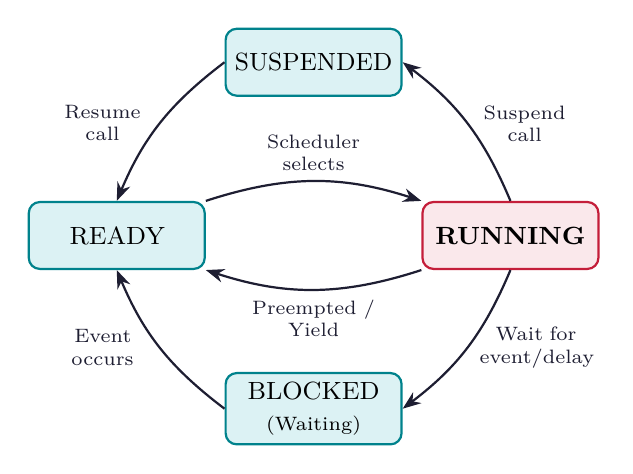
\begin{tikzpicture}[
  tstate/.style={rectangle, draw=myteal, fill=hdrteal, text width=2.0cm,
    align=center, minimum height=0.85cm, font=\small, rounded corners=4pt, line width=0.8pt},
  rstate/.style={rectangle, draw=myred, fill=hdrred, text width=2.0cm,
    align=center, minimum height=0.85cm, font=\small\bfseries, rounded corners=4pt, line width=0.8pt}]

  \node[tstate] (ready)     at (0,   0)    {READY};
  \node[rstate] (running)   at (5,   0)    {RUNNING};
  \node[tstate] (blocked)   at (2.5, -2.2) {BLOCKED \\ \scriptsize(Waiting)};
  \node[tstate] (suspended) at (2.5,  2.2) {SUSPENDED};

  \draw[arrow] (ready.north east) to[bend left=18]
    node[above, font=\scriptsize, align=center] {Scheduler \\ selects} (running.north west);
  \draw[arrow] (running.south west) to[bend left=18]
    node[below, font=\scriptsize, align=center] {Preempted / \\ Yield} (ready.south east);
  \draw[arrow] (running.south) to[bend left=15]
    node[right, font=\scriptsize, align=center, text width=1.5cm] {Wait for \\ event/delay} (blocked.east);
  \draw[arrow] (blocked.west) to[bend left=15]
    node[left, font=\scriptsize, align=center, text width=1.2cm] {Event \\ occurs} (ready.south);
  \draw[arrow] (running.north) to[bend right=15]
    node[right, font=\scriptsize, align=center, text width=1.2cm] {Suspend \\ call} (suspended.east);
  \draw[arrow] (suspended.west) to[bend right=15]
    node[left, font=\scriptsize, align=center, text width=1.2cm] {Resume \\ call} (ready.north);
\end{tikzpicture}
\end{tcolorbox}


\subsection{Task Scheduling Algorithms}

\subsubsection*{1. Priority-Based Preemptive Scheduling}

\begin{tcolorbox}[defbox, title={\textbf{Priority-Based Preemptive Scheduling}}]
Each task is assigned a \textbf{priority} (numeric value). The scheduler always runs the highest-priority task that is in the READY state. If a higher-priority task becomes ready while a lower-priority task runs, the lower-priority task is \textbf{immediately preempted} (stopped) and the higher-priority task takes the CPU.
\end{tcolorbox}

\begin{itemize}[leftmargin=*, itemsep=3pt]
  \item \textbf{Deterministic:} Highest-priority tasks always respond within bounded time.
  \item \textbf{Starvation risk:} Very low-priority tasks may never run if higher-priority tasks are always ready.
  \item \textbf{Priority Inversion:} A high-priority task is blocked because a low-priority task holds a shared resource. Solved by \textbf{Priority Inheritance Protocol}.
  \item \textbf{Used in:} FreeRTOS, VxWorks, RTEMS, most industrial RTOS.
\end{itemize}

\subsubsection*{2. Cyclic Scheduling (Time-Division Multiplexing)}

\begin{tcolorbox}[defbox, title={\textbf{Cyclic Scheduling}}]
Tasks are arranged in a \textbf{fixed cyclic sequence} (also called a \textbf{static schedule}). A major cycle (hypercycle) is divided into \textbf{time slots}, and each task runs during its assigned slot. No dynamic priority decisions --- the schedule is fixed at design time.
\end{tcolorbox}

\begin{itemize}[leftmargin=*, itemsep=3pt]
  \item \textbf{Predictable:} Exact execution times are known at compile time.
  \item \textbf{Simple:} No complex scheduler overhead.
  \item \textbf{Inflexible:} Cannot respond to dynamic events; hard to add new tasks.
  \item \textbf{Used in:} Safety-critical aerospace and automotive systems (ARINC 653, AUTOSAR).
\end{itemize}

\subsubsection*{3. Round-Robin Scheduling}

\begin{tcolorbox}[defbox, title={\textbf{Round-Robin Scheduling}}]
All tasks of \textbf{equal priority} are given equal CPU time \textbf{time slices} (quantum, e.g., 10 ms). The scheduler cycles through all ready tasks in a circular queue. When a task's time slice expires, it is preempted and the next task in the queue runs.
\end{tcolorbox}

\begin{itemize}[leftmargin=*, itemsep=3pt]
  \item \textbf{Fair:} All equal-priority tasks share CPU time equally.
  \item \textbf{No starvation} for equal-priority tasks.
  \item \textbf{Response time:} Depends on the number of tasks and the time quantum (worst case: $(n-1) \times Q$).
  \item \textbf{Used in:} Linux time-sharing, RTOS task groups at same priority.
\end{itemize}

\subsection{Comparison of RTOS Scheduling Algorithms}

\par\noindent
{\renewcommand{\arraystretch}{1.55}%
\begin{tabularx}{\linewidth}{|B{3.0cm}|Y|Y|Y|}
\hline
\textbf{Feature} & \textbf{Priority-Based} & \textbf{Cyclic} & \textbf{Round-Robin} \\
\hline
\textbf{Flexibility} & High & Low & Medium \\
\hline
\textbf{Determinism} & High & Very High & Medium \\
\hline
\textbf{Fairness} & Low (priority skew) & Fixed & High (equal priority) \\
\hline
\textbf{Overhead} & Medium & Very Low & Low \\
\hline
\textbf{Starvation} & Possible & No & No (equal priority) \\
\hline
\textbf{Best For} & General RTOS & Safety-critical & Time-sharing tasks \\
\hline
\end{tabularx}}

\subsection{Basic Design Rules Using RTOS}
\begin{enumerate}[label=\textbf{\arabic*.}, leftmargin=*, itemsep=4pt]
  \item \textbf{Assign priorities carefully:} Critical, fast-response tasks (e.g., motor control) get the highest priority. Background tasks (e.g., logging) get the lowest.
  \item \textbf{Use semaphores/mutexes} to protect shared resources (global variables, hardware peripherals) from concurrent access by multiple tasks.
  \item \textbf{Avoid blocking calls in high-priority tasks:} Use non-blocking APIs or timeouts.
  \item \textbf{Minimize stack usage:} Each task has its own stack. Over-allocating wastes RAM; under-allocating causes stack overflow (hard to debug).
  \item \textbf{Keep ISRs minimal:} ISR sets a flag or sends to a queue; task processes the data.
  \item \textbf{Use RTOS trace tools:} Tools like FreeRTOS+Trace or Segger SystemView to observe task switching, timing, and CPU usage.
\end{enumerate}

% ===============================================================================
% MANDATORY QUICK REVISION PAGE
% ===============================================================================
\newpage
\begin{center}
  {\large\bfseries\color{myred} Quick Revision --- Module 4}\\[3pt]
  {\small\color{mydark} Embedded Software Development \& RTOS $|$ PE-EC703A}
\end{center}
\noindent{\color{myred}\rule{\linewidth}{1.2pt}}
\vspace{4pt}

\begin{tcolorbox}[formulabox, title={\textbf{Key Formulas at a Glance}}]
\renewcommand{\arraystretch}{1.3}
\begin{tabularx}{\linewidth}{B{4.5cm} X}
8051 Delay Loop Cycles & $N_{cycles} = (\text{count}_{outer}) \times (\text{count}_{inner}) \times 5$ (approx., per DJNZ) \\[4pt]
RTOS Response Time (RR) & $t_{response} \leq (n - 1) \times Q$ \quad ($n$ = tasks at same priority, $Q$ = time quantum) \\[4pt]
CPU Utilization Check & $U = \displaystyle\sum_{i=1}^{n} \frac{C_i}{T_i} \leq 1$ \quad ($C_i$ = exec. time, $T_i$ = period of task $i$)
\end{tabularx}
\end{tcolorbox}

\begin{tcolorbox}[defbox, title={\textbf{One-Line Definitions}}]
\begin{itemize}[leftmargin=*, itemsep=2.5pt, topsep=0pt]
  \item \textbf{ALP:} Assembly Language Programming --- low-level mnemonic-based programming for direct hardware control.
  \item \textbf{Assembler:} Translates assembly (mnemonic) code to binary machine code.
  \item \textbf{Cross-compiler:} Compiler on a host PC generating code for a different target (e.g., ARM GCC).
  \item \textbf{volatile:} C keyword that prevents compiler from caching a variable that can change externally (e.g., ISR flag).
  \item \textbf{Preprocessor Directive:} Instructions beginning with \texttt{\#} that control compilation before the compiler runs.
  \item \textbf{Inline function:} C++ function expanded at call site by the compiler, eliminating function call overhead.
  \item \textbf{RTOS:} Operating system guaranteeing deterministic task scheduling with hard timing deadlines.
  \item \textbf{Task (Thread):} An independent unit of execution managed by the RTOS scheduler.
  \item \textbf{Preemption:} RTOS forcibly stopping a running task to run a higher-priority task.
  \item \textbf{Semaphore:} RTOS signaling mechanism for synchronization between tasks or between ISR and tasks.
  \item \textbf{Mutex:} Mutual exclusion object; protects shared resources from concurrent access (includes priority inheritance).
  \item \textbf{Priority Inversion:} A high-priority task blocked by a low-priority task holding a needed resource.
  \item \textbf{Round-Robin:} Scheduling algorithm giving equal time slices to all tasks at the same priority level.
\end{itemize}
\end{tcolorbox}

\begin{tcolorbox}[exambox, title={\textbf{Frequently Asked / Viva Questions}}]
\begin{enumerate}[topsep=0pt, label=\textbf{Q\arabic*.}, itemsep=5pt]
  \item \Q{What is the difference between assembly language and C for embedded programming?}
    ALP gives maximum hardware control, exact cycle-count timing, and minimum code size but is processor-specific and harder to maintain. C provides portability, structured code, and faster development with slightly larger code. Both are commonly mixed: C for application logic, ALP for startup and timing-critical routines.
  \item \Q{What is the purpose of the \texttt{volatile} keyword in embedded C?}
    It tells the compiler that a variable can change unexpectedly (by an ISR, DMA, or hardware register) and must not be optimized or cached. Without \texttt{volatile}, the compiler may read the variable once and reuse the cached value, missing updates.
  \item \Q{What are preprocessor directives? Give two examples.}
    Instructions beginning with \texttt{\#} that are processed before compilation. Examples: \texttt{\#define LED 5} (macro constant), \texttt{\#include "stm32.h"} (file inclusion), \texttt{\#ifdef DEBUG} (conditional compilation).
  \item \Q{What is an RTOS and how does it differ from a bare-metal embedded system?}
    An RTOS provides multi-tasking, scheduling, and synchronization services. In bare-metal, a single \texttt{while(1)} loop and ISRs handle everything sequentially --- no time guarantees between events. RTOS ensures tasks run within defined deadlines and can run concurrently.
  \item \Q{Explain priority-based preemptive scheduling.}
    Each task has a priority number. The RTOS scheduler always runs the highest-priority READY task. If a higher-priority task becomes ready (e.g., unblocked by an ISR posting to its queue), the currently running lower-priority task is immediately preempted and the higher-priority task takes the CPU.
  \item \Q{What is priority inversion and how is it solved?}
    Priority inversion: a high-priority task (H) is blocked waiting for a resource held by a low-priority task (L), while a medium-priority task (M) runs and prevents L from completing. \textbf{Solution:} Priority Inheritance --- temporarily raise L's priority to H's level until it releases the resource.
  \item \Q{Compare cyclic scheduling and round-robin scheduling.}
    Cyclic scheduling uses a fixed time-division slot sequence (fully deterministic, best for safety-critical systems, inflexible). Round-robin dynamically gives equal time quantum to all equal-priority tasks (fair, flexible, slight unpredictability in deadline, good for general tasks).
  \item \Q{What is the difference between a semaphore and a mutex?}
    A \textbf{semaphore} is a signaling mechanism (binary or counting) primarily used for task synchronization and ISR-to-task signaling. A \textbf{mutex} (Mutual Exclusion) is specifically for protecting shared resources from concurrent access and includes priority inheritance to prevent priority inversion.
  \item \Q{What is the role of the RTOS kernel?}
    The RTOS kernel manages task creation, deletion, scheduling (context switching), inter-task communication (queues, semaphores), timers, and memory allocation. It runs the context switch code that saves and restores task registers during task switching.
  \item \Q{What are the advantages of C++ over C in embedded programming?}
    C++ provides encapsulation (classes for peripheral drivers), type safety (templates), compile-time computation (constexpr), and RAII for automatic resource management. These improve code organization and reliability with zero runtime cost if high-overhead features (exceptions, RTTI, heap) are avoided.
  \item \Q{What is a time quantum in round-robin scheduling?}
    The time quantum (slice) is the maximum CPU time a task runs before being preempted and the next task getting a turn. Shorter quantum gives better responsiveness but more context-switch overhead. Typical values: 1--20 ms.
  \item \Q{What is the \texttt{DJNZ} instruction in 8051 assembly and why is it used?}
    \texttt{DJNZ Rn, label} --- Decrement Register $n$ and Jump if Not Zero. It is the standard loop instruction: \texttt{MOV R0, \#100; LOOP: DJNZ R0, LOOP} creates a 100-iteration delay loop with a 2-machine-cycle instruction --- very efficient for timing loops.
\end{enumerate}
\end{tcolorbox}

\begin{tcolorbox}[tikzbox, title={RTOS Scheduling: Priority-Based vs.\ Round-Robin Timeline}]
\centering
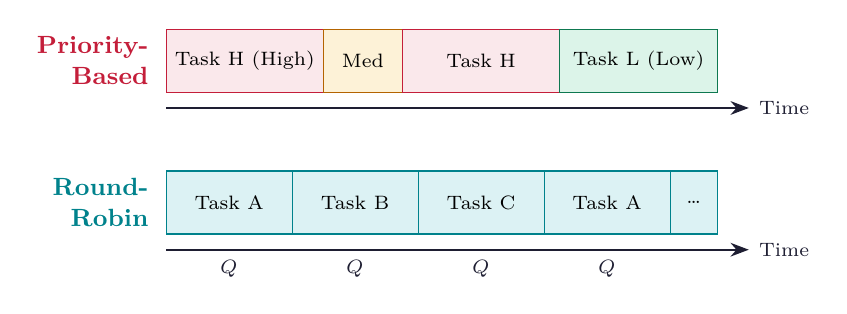
\begin{tikzpicture}[every node/.style={font=\small}]
  % ── Priority-Based row (y = 2.2 – 3.0) ──
  \node[left, align=right, font=\small\bfseries\color{myred}] at (2.5, 2.6) {Priority-\\Based};
  \draw[fill=hdrred,   draw=myred]   (2.6, 2.2) rectangle (4.6, 3.0) node[midway, font=\scriptsize] {Task H (High)};
  \draw[fill=hdramber, draw=myamber] (4.6, 2.2) rectangle (5.6, 3.0) node[midway, font=\scriptsize] {Med};
  \draw[fill=hdrred,   draw=myred]   (5.6, 2.2) rectangle (7.6, 3.0) node[midway, font=\scriptsize] {Task H};
  \draw[fill=hdrgreen, draw=mygreen] (7.6, 2.2) rectangle (9.6, 3.0) node[midway, font=\scriptsize] {Task L (Low)};
  \draw[-Stealth, color=mydark, thick] (2.6, 2.0) -- (10.0, 2.0) node[right, font=\scriptsize] {Time};

  % ── Round-Robin row (y = 0.4 – 1.2) ──
  \node[left, align=right, font=\small\bfseries\color{myteal}] at (2.5, 0.8) {Round-\\Robin};
  \draw[fill=hdrteal, draw=myteal] (2.6, 0.4) rectangle (4.2, 1.2) node[midway, font=\scriptsize] {Task A};
  \draw[fill=hdrteal, draw=myteal] (4.2, 0.4) rectangle (5.8, 1.2) node[midway, font=\scriptsize] {Task B};
  \draw[fill=hdrteal, draw=myteal] (5.8, 0.4) rectangle (7.4, 1.2) node[midway, font=\scriptsize] {Task C};
  \draw[fill=hdrteal, draw=myteal] (7.4, 0.4) rectangle (9.0, 1.2) node[midway, font=\scriptsize] {Task A};
  \draw[fill=hdrteal, draw=myteal] (9.0, 0.4) rectangle (9.6, 1.2) node[midway, font=\scriptsize] {\ldots};
  \draw[-Stealth, color=mydark, thick] (2.6, 0.2) -- (10.0, 0.2) node[right, font=\scriptsize] {Time};
  % Q markers at each slot boundary
  \foreach \x in {3.4, 5.0, 6.6, 8.2} {
    \node[below, font=\scriptsize, color=mydark] at (\x, 0.2) {$Q$};
  }
\end{tikzpicture}
\end{tcolorbox}

\end{document}
